% https://www.grund-wissen.de/informatik/latex/mathematischer-formelsatz.html
% https://docplayer.org/28012320-Mathematische-formelsammlung.html
% add CC license
% use Command+Shift+Click in the PDF to jump to the source code line when using TeXShop

%
\author{Dirk~Messetat}
\date{\today}
\newcommand{\versionsnummer}{1.0.0-SNAPSHOT}

% URL:
\newcommand{\url}{}

% Titel:
\title{Mathematische \\
FORMELSAMMLUNG \\[2ex] \small Version: \versionsnummer \\[2ex] \texttt{ \url{http://github.com/codirk/formelsamlung} }\\
 \hfill\break
Klasse 5-13
}

\documentclass[12pt,a4paper,fleqn,twoside,pdf,final]{scrartcl}
%\documentclass[12pt,a4paper,fleqn,twoside,pdf,final]{article}
%\documentclass{scrartcl}


\usepackage{graphicx}


\usepackage[ngerman]{babel}
\usepackage[utf8]{inputenc}
% \usepackage[T1]{fontenc}


\setlength{\parindent}{0in}
\setlength{\mathindent}{0pt}

\usepackage{amsfonts}


\usepackage{helvet}
\usepackage{curves}
\usepackage{latexsym}
\usepackage{textcomp}

% damages the pictures
%\usepackage[dvips]{rotating}

\usepackage{geometry}

\geometry{left=0.5cm,textwidth=19cm,top=1.0cm,textheight=26cm}

\usepackage{array}

%\usepackage{creativecommons}
\usepackage[hidelinks]{hyperref}

\usepackage[
    type={CC},
    modifier={by-nc-sa},
    version={3.0},
]{doclicense}


% striked out text
\usepackage[normalem]{ulem}
\usepackage{cancel}

\usepackage{framed}
\usepackage{listings}
\usepackage{graphicx}
\usepackage{textcomp}
\usepackage{tikz}
\usepackage{tikz-qtree}
\usetikzlibrary{shapes,automata,arrows}
\usepackage{pgfplots}
\usepackage{color}




\usepackage{amsmath}
%\usepackage[draft]{graphics} % ohne Bilder (Entwurf)
\usepackage{graphics} % Bilder einbinden

\nonfrenchspacing
\renewcommand{\familydefault}{\sfdefault}


% newcommand
\newcommand{\stkout}[1]{\ifmmode\text{\cancel{\ensuremath{#1}}}\else\sout{#1}\fi}

\usepackage{float}
\usepackage{subfig}

\usetikzlibrary{calc,angles}
\usetikzlibrary{shapes,arrows,intersections}
\usetikzlibrary{matrix,fit,calc,trees,positioning,arrows,chains,shapes.geometric,shapes,angles}
\usetikzlibrary{quotes}

%\usetikzlibrary{calc,angles,quotes}
\tikzset{square/.style= { to path={ let \p1=(\tikztostart), \p2=(\tikztotarget),
  \p3=($(\p2)!1!90:(\p1)$), \p4=($(\p1)!1!-90:(\p2)$) in
  (\p2) foreach \i in {3,4,1,2} {--node[auto=right]{#1} (\p\i)}}}}

\usepackage{siunitx}


\documentclass{formulaCollection}

\RequirePackage{formulaCollection}

%TODO Print this message during the build

\setlength{\parindent}{0in}
\setlength{\mathindent}{0pt}

\graphicspath {{./sections/}{./sections/08_Geometrie/}}



\begin{document}


\maketitle
\thispagestyle{empty}


% Fill with blanks to bottom of first page
\vfill
 

%\begin{flushright}
%    \copyright  2021 Dirk Messetat git [at] messetat [dot] com. \\ 
%    This work is licensed under a Creative Commons Attribution- ShareAlike 3.0 License.
%    To view a copy of this license visit:
%     \url{http://creativecommons.org/licenses/by-sa/3.0/legalcode}.
%\end{flushright}

%default:\quad
%\qrcode{https://www.ctan.org/tex-archive/macros/latex/contrib/qrcode?lang=en}
%\qquad
%1 inch high (and wide):
%\quad

\begin{center}
Wer keine Formeln schreibt, braucht sich damit nicht zu beschäftigen.
\end{center}

% \centering{Wer keine Formeln schreibt, braucht sich damit nicht zu beschäftigen.}


% this works with pdflatex but not with latex
%\doclicenseThis




\pagebreak



% Inhaltsverzeichnis
\setcounter{tocdepth}{1}
\tableofcontents
\thispagestyle{empty}


\vfill

\begin{center}
\small{Dieses Dokument wurde mit \LaTeX{} gesetzt.}
\end{center}

\newpage

\clearpage
\pagenumbering{arabic} 

%% https://de.wikipedia.org/wiki/Liste_mathematischer_Symbole

\section{Mengenlehre}

\subsection{Mengenverknüpfung}

\begin{tabular}[h]{lll}

% The symbols \land, \lor and \lnot have synonyms: \wedge, \vee and \neg
Symbol &Menge & Formel \\
\hline
$\cup$ & Vereinigungsmenge	 & \{$x \in M \lor x \in N$\} \\
$\cap$ & Schnittmenge	 & \{$x \in M \land x \in N$\} \\
$\setminus$ & Differenzmenge	 & \{$x \in M \land x \notin N$\} \\
$\triangle$ & Symmetrische Differenz & \{TBD\} \\
$\times$ & Kartesisches Produkt & \{TBD\} \\
$\dot\cup$ & Vereinigung disjunkter Mengen  & \{TBD\} \\
$\sqcup$ & Disjunkte Vereinigung der Mengen  & \{TBD\} \\
$\bar{A}$ & Komplement & \{TBD\} \\
$\mathcal{P}$ & Potenzmenge & \{TBD\} \\
\end{tabular}

\subsection{Characteristische Mengen}

\begin{tabular}[h]{lll}
Symbol &Menge & Beispiele \\
\hline
$\emptyset$ & leere Menge & \{\} \\
$\mathbb{P}$ & Primzahlen & \{2,3,5,7,11,13,...\} \\
$\mathbb{N}$ & Natürliche Zahlen & \{1,2,3,...\} \\
$\mathbb{N}_0$ & Natürliche Zahlen mit 0 & \{0,1,2,3,..\} \\
$\mathbb{Z}$ & Ganze Zahlen & \{..,-3,-2,-1,0,1,2,3,...\} \\
$\mathbb{Z}^+$ & Ganze Zahlen & \{1,2,3,..\} \\
$\mathbb{Z}^-$ & Ganze Zahlen & \{...,-3,-2,-1\} \\
$\mathbb{Q}$ & Rationale Zahlen & \{ $\frac{p}{q} | (p \in \mathbb{Z}) \wedge (q \in  \mathbb{Z} \setminus \{0 \} ) $ \} \\
$\mathbb{I}$ & Irrationale Zahlen & \{$\sqrt{2},\pi, e,...$\} \\
$\mathbb{R}$ & Reelle Zahlen & $\mathbb{R} \cup \mathbb{I}$\\
$\mathbb{T}$ & Transzendente Zahlen & \{ $\pi, e$ \} \\
$\mathbb{C}$ & Komplexe Zahlen & \{ $x + iy | x,y \in \mathbb{R} $\} \\
\end{tabular}

\subsection{Teilbarkeitsregeln (natürliche Zahlen)}
Ist a durch t ohne Rest teilbar?\\
$t|a$ t teilt a


$t=2$ wenn die letzte Ziffer eine durch 2 teilbare Zahl darstellt\\
$t=3$ wenn die Quersumme durch 3 teilbar ist\\
$t=4$ wenn die letzten \textbf{zwei} Ziffern eine durch 4 teilbare Zahl bilden\\
$t=5$ wenn die letzte Ziffer eine durch 5 teilbare Zahl darstellt\\
$t=6$ wenn die Zahl durch 2 und 3 teilbar ist\\
$t=7$ (Für die Zahl 7 gibt es keine einfache Teilbarkeitsregel!)\\
$t=8$ wenn die letzten \textbf{drei} Ziffern eine durch 8 teilbare Zahl bilden\\
$t=9$ wenn die Quersumme durch 9 teilbar ist\\
$t=10$ wenn die letzte Ziffer eine 0 ist

Komplexere Regeln \\
$t=7$ wenn die alternierende 3er-Quersumme durch 7 teilbar ist\\
$t=11$ wenn die alternierende Quersumme durch 11 teilbar ist\\
$t=13$ wenn die alternierende 3er-Quersumme durch 11 teilbar ist


\subsection{Quersummenregeln}
\subsubsection{Quersumme}
$Q(1234)=4+3+2+1=10$

\subsubsection{Alternierende Quersumme}

$Q^{\prime}(1234)=4-3+2-1=2$\\
$Q^{\prime}(4321)=1-2+3-4=-1$\\
$Q^{\prime}(3223)=3-2+2-3=0$\\
$Q^{\prime}(68786979)=9+9+8+8-(7+6+7+6)=34-26=8$




\subsection{Intervalle}

\begin{align*}
[a,b]  &=  \{x| a \leq x \leq b, x \in \mathbb{R}\} \\
(a,b) &= ]a,b[ =  \{x| a <  x < b, x \in \mathbb{R}\} \\
[a,b) &= [a,b[ =  \{x| a \leq  x < b, x \in \mathbb{R}\} \\
(a,b] &= ]a,b] =  \{x| a <  x \leq b, x \in \mathbb{R}\}
\end{align*}
\subimport*{sections/}{01_Mengenlehre}

\pagebreak
\section{Arithmetik}
\subsection{Brüche}

Kürzen:
\begin{align*}
\frac{ac}{bc} = \frac{a \cdot c}{b \cdot c} =  \frac{a \cdot c : c }{b \cdot c : c} =  \frac{a \cdot 1 }{b \cdot 1 } =  \frac{a \cdot \stkout{c} }{b \cdot \stkout{c}}  =  \frac{a}{b}  
\end{align*}

Erweitern:
\begin{align*}
\frac{a}{b} =  \frac{ac}{bc} =   \frac{a \cdot c}{b \cdot c} 
\end{align*}

Addition und Subtraktion gleichnamiger Brüche:

\begin{align*}
  \frac{a}{c} \pm \frac{b}{c} =  \frac{a \pm b}{c} 
\end{align*}

Addition und Subtraktion nicht gleichnamiger Brüche:

\begin{flalign*}
\frac{a}{b} \pm \frac{c}{d} &= \frac{ad}{bd} \pm \frac{cb}{db} = \frac{ad \pm bc}{db} \\
\Rightarrow \frac{a}{b} \pm c &= \frac{a}{b} \pm \frac{c}{1} = \frac{a \pm bc}{b} 
\end{flalign*}


Multiplikation Bruch:
\begin{align*}
\frac{a}{b} c = c \frac{a}{b} = \frac{a}{b} \cdot c = \frac{a}{b}  \cdot \frac{c}{1}  = \frac{a \cdot c}{b \cdot 1} = \frac{a \cdot c}{b}  = \frac{a c}{b} 
\end{align*}

Achtung! : Addition bei Zahlen
\begin{align*}
2\frac{1}{3} = 2+\frac{1}{3} =  \frac{6}{3} + \frac{1}{3} = \frac{7}{3} 
\end{align*}



Division Bruch mit Bruch (Multiplikation mit Kehrwert):
\begin{flalign*}
\frac{a}{b} : \frac{c}{d}&= \frac{a}{b} \cdot \frac{d}{c}= \frac{a \cdot d }{b \cdot c}= \frac{a d }{b c} \\
\Rightarrow \frac{a}{b}:c&= \frac{a}{b} : \frac{c}{1}=\frac{a}{b} \cdot \frac{1}{c}=\frac{a}{b \cdot c}  = \frac{a}{b c} 
\end{flalign*}


\pagebreak
\subsection{Klammerrechnung}

Addition von Summanden (assoziativ):
\begin{align*}
 a + (b \pm c) = (a + b) \pm c = a + b \pm c 
\end{align*}
Subtraction von Summanden:
\begin{align*}
 a - (b \pm c) = a + (-1) \cdot  (b \pm c) = a + (  (-1) \cdot  b \pm  (-1) \cdot c)  =  a - b \mp c
\end{align*}


Multiplikation mit Summe:
\begin{align*}
 a (b \pm c) =  a \cdot (b \pm c) = a \cdot b \pm a \cdot c = ab \pm ac
\end{align*}
Bzw.
\begin{align*} 
 \sum_{i=1}^n ax_{i}  = a \cdot  \sum_{i=1}^n x_{i} = a  \sum_{i=1}^n x_{i}
 \end{align*}


Multiplikation von Summen:
\begin{align*}
 (a+b)(b+c) = a \cdot c +a \cdot d +b \cdot c +b \cdot d = ac +ad +bc +bd 
\end{align*}

Division einer Summe:
\begin{align*}
 (a \pm b):(c) = \frac{a \pm b}{c} = \frac{a}{c} \pm  \frac{b}{c} 
\end{align*}

\subsection{Binomische Formeln}
\begin{align*}
(a+b)^ 2 = a^ 2 + 2ab + b^2\\
(a-b)^ 2 =  a^ 2 - 2ab + b^2 \\
(a+b)(a-b) = a^ 2 - b^2
\end{align*}
 

%
$a^ 2 + b^2 $ (reell nicht zerlegbar!) 

\begin{align*} 
a^ 3 + b^3 = (a+b)( a^ 2 - ab + b^2) \\
a^ 3 - b^3 = (a-b)( a^ 2 + ab + b^2)
\end{align*}


\begin{tabular}{>{$n=}l<{$\hspace{12pt}}*{14}{c}}
0 &&&&&&&1&&&&&&& $(a+b)^ 0=1$\\
1 &&&&&&1&&1&&&&&& $(a+b)^ 1=1a+1b$ \\
2 &&&&&1&&2&&1&&&&&  $(a+b)^ 2=1a^ 2+2ab+1b^2$\\
3 &&&&1&&3&&3&&1&&&& $(a+b)^ 3=1a^3+3a^2 b+3ab^2+1b^3$\\
4 &&&1&&4&&6&&4&&1&&& $(a+b)^ 4=a^4+4a^3 b+6a^2b^2+4ab^3+b^4$\\
5 &&1&&5&&10&&10&&5&&1&&\\
6 &1&&6&&15&&20&&15&&6&&1&
\end{tabular}

Binominalkoeffizienten (n über k)
\begin{align*}
\binom{n}{k}= \frac{n(n-1)(n-2)...[n-(k-1)] }{k!} =  \frac{n!}{k!(n-k)!}
\end{align*}


\begin{align*}
n! = 1\cdot2\cdot3...(n-1)n= \prod_{k = 1}^{n}k    (n \in \mathbb{N})
\end{align*}





\subsection{Potenzen}
Potenz eines Produktes gleicher Grundzahl: 
$a^m \cdot a^n = a^{m+n}$

Potenz einer Division/Bruches gleicher Grundzahl: $ \frac{a^m}{a^n} = a^{m-n}$ \\
$\longrightarrow$ $ a^0 =  \frac{a^n}{a^n} =   \frac{ \cancel{a^n} \cdot 1}{ \cancel{a^n} \cdot 1} = a^{n-n}  = 1$  ; $a \in \{a| a \neq 0\}$ \\
$\longrightarrow$ negative Exponenten: $ a^{-n} =  a^{0-n} =  \frac{a^0}{a^n}  =  \frac{1}{a^n} $ \\

Potenz eines Produktes mit gleichen Exponenten: $ {a^n}{b^n} = (ab)^{n}$ 

Potenz einer Division/Bruches mit gleichen Exponenten: $ \frac{a^n}{b^n} = (\frac{a}{b}) ^n$ 

Potenz einer Potenz: $ (a^m)^n = a^{m^n} = a^{m \cdot n}$ 

Potenz von 0: $ 0^n = 0 $ ;  $n \in\{n | n > 0\}$\\
Potenz 0 von 0: $ 0^0 = foobar $ 

\subsection{Wurzeln}

Radizieren eines Produktes $\sqrt[n]{ab} = \sqrt[n]{a} \cdot \sqrt[n]{b}$

Radizieren eines Quotienten $\sqrt[n]{\frac{a}{b} } = \frac{\sqrt[n]{a}}{\sqrt[n]{b}} $

Radizieren einer Potenz $\sqrt[n]{ a^m} = (\sqrt[n]{ a})^m = a^{\frac{m}{n}}$

Radizieren einer Wurzel $\sqrt[n]{\sqrt[m]{a}}  = \sqrt[n \cdot m]{a} = \sqrt[m]{\sqrt[n]{a}}$


\subsection{Logarithmen}
$$ b^x =n \longleftrightarrow x = \log_b n$$

Logarithmieren eines Produktes $\log_b (m \cdot n) = \log_b m + \log_b n $ 

Logarithmieren eines Quotienten $\log_b (\frac{m}{n}) = \log_b m - \log_b n  $ 

Logarithmieren einer Potenz $\log_b (m^n) =  n \cdot \log_b m $ 

Logarithmieren einer Wurzel $\log_b (\sqrt[n]{m}) =  \frac{1}{n} \cdot \log_b m $ 

Logarithmentsysteme \\
$\log_{10} n = \lg n $\\
$\log_{e} n = \ln n $


\section{Algebra}
\subsection{Gesetze}
Kommutativgesetz:Vertauschungsgesetz \\
Assoziativgesetz: Verknüpfungsgesetz oder auch Verbindungsgesetz (Klammern verschieben) \\
Distributivgesetz: Verteilungsgesetze (Ausklammern/Ausmultiplizieren)






% \subsection{Ungleichungen}

\subsection{Gleichungen}
Äquivalenzumformungen (T $\widehat{=}$ Term)
\begin{align*}
T_1 &= T_2 &\longrightarrow& & T_2 &= T_1 \\
T_1 &= T_2 | \pm T_3 &\longrightarrow& & T_1 \pm T_3 &= T_2 \pm T_3 \\
T_1 &= T_2 | \cdot a &\longrightarrow& & T_1 \cdot a &= T_2 \cdot a &a \in \{a|a \neq 0\} \\
T_1 &= T_2 | : a &\longrightarrow& & \frac{T_2}{a} &= \frac{T_2}{a} &a \in \{a|a \neq 0\} \\
\end{align*}


\subsubsection{Linieare Gleichungen}

\paragraph{2 Gleichungen mit 2 Unbekannten}

\begin{align*}
a x + by - c = 0\\
d x + e y - f = 0\\
oder \\
a_{11} x_1 + a_{12} x_2 - K_1 = 0\\
a_{21} x_1 + a_{22} x_2 - K_2 = 0\\
\end{align*}

\subparagraph{Determinaten}
\begin{align*}
D= a_{11} a_{22} - a_{12} a_{21} = \left|
    \begin{array}{ccc}
       a_{11} & a_{12} \\
       a_{21} & a_{22} \\
    \end{array}
    \right|
\end{align*}

\begin{align*}
D_{{x}_1}= K_1 a_{22} - K_2 a_{12} = \left|
     \begin{array}{ccc}
        K_1 & a_{12} \\
        K_2 & a_{22} \\
     \end{array}
     \right|
\end{align*}

\begin{align*}
D_{{x}_2}= K_2 a_{11} - K_1 a_{21} = \left|
     \begin{array}{ccc}
        a_{11} & K_1 \\
        a_{21} & K_2 \\
     \end{array}
     \right|
\end{align*}

\subparagraph{Cramer'sche Regel}
Wenn alle Gleichungen linear unabhängig sind
\begin{align*}
D &\neq 0
\end{align*}
dann
\begin{align*}
x_1 &= \frac{ D_{{x}_1} }{D} \\
x_2 &= \frac{ D_{{x}_2} }{D} \\
\end{align*}



\paragraph{m-Gleichungen mit n-Unbekannten}
Die Cramer'sche Regel gild analog für m Gleichungen mit n Variablen.
\begin{align*}
a_{11}x_{1}+a_{12}x_{2}+a_{13}x_{1}+...+a_{1n}x_{2}-c_{1}&=0 \\
a_{21}x_{1}+a_{22}x_{2}+a_{23}x_{1}+...+a_{2n}x_{2}-c_{1}&=0 \\
a_{31}x_{1}+a_{32}x_{2}+a_{33}x_{1}+...+a_{3n}x_{2}-c_{1}&=0 \\
...\\
a_{m1}x_{1}+a_{m2}x_{2}+a_{m3}x_{1}+...+a_{mn}x_{2}-c_{m}&=0 \\
\end{align*}

\subparagraph{Determinaten}
$$
D=\left|
\begin{array}{ccc}
   a_{11} & \cdots & a_{1n} \\
   \vdots & \ddots & \vdots \\
   a_{n1} & \cdots & a_{nn}
\end{array}
\right|
$$



\subsection{Quadratische Gleichungen}
Allgemeine Form:
$ ax^2 + bx + c = 0 $

Normalform:
$ x^2 + px + q = 0 $ mit $p=\frac{b}{a}$ und $q=\frac{c}{a}$

Lösung: $x_{1,2}= - \frac{p}{2} \pm \sqrt[]{( \frac{p}{2})^2 -q }$

Linearfactoren (Produktform quadratischer Terme): $(x-x_1)\cdot (x-x_2 )=0$

\subsection{Polynomfunktion n-ten Grades}
Ein Polynom n-ten Grades lässt sich maximal in n Linearfaktoren zerlegen und hat maximal n Lösungen bzw. hat maximal n Nullstellen.
\begin{align*}
f(x) &= a_nx^n+a_{n-1}x^{n-1}+...+a_1x^1+a_0 \\
p(x) &=a_n(x-n_1)(x-n_2)(x-n_3)...(x-n_N) \textrm{ mit jeweils den Nullstellen } n_k
\end{align*}

\pagebreak
\section{Relationen und Funktionen}

\section{Folgen und Reihen}
\subsection{Arithmetische Folgen und Reihen}

\begin{align*}
d &=a_{n+1} - a_n = const. ; n \in \mathbb{N}
\end{align*}

\paragraph{Arithmetisches Mittel}
\begin{align*}
    a_n=\frac{a_{n-1}+a_{n+1}}{2}
\end{align*}

\paragraph{Funktionsforschrift}
\begin{align*}
    a_n = a_1+(n-1) \cdot d ; d \in \{d|d \neq 0\}
\end{align*}

\paragraph{Summenformel}
\begin{align*}
    \sum_{k=1}^{n} a_k &= \frac{a_1+a_n}{2} \cdot n \\
    &= \sum_{k=1}^{n} a_1 +(k-1) \cdot d \\
    &= \frac{n}{2}[2a_1+(n-1) \cdot d]
\end{align*}



\subsection{Geometrische Folgen und Reihen}
\begin{align*}
    q = \frac{a_{n+1}}{a_n} = const. ; a_n \neq 0
\end{align*}

\paragraph{Geometrisches Mittel}
\begin{align*}
    a_n= \sqrt{a_{n-1} \cdot a_{n+1}}
\end{align*}

\paragraph{Funktionsforschrift}
\begin{align*}
    a_n = a_1 \cdot q^{n-1} ; q \in \{q | q \neq 0\}
\end{align*}

\paragraph{Summenformel}
\begin{align*}
    \sum_{k=1}^{n} a_k &= \sum_{k=1}^{n} a_1 \cdot q^{k-1}\\
    &= a_1 \frac{q^n-1}{q-1} ; \textrm{für} |q| > 1\\
    &= a_1 \frac{1-q^n}{1-q} ; \textrm{für} |q| < 1
\end{align*}

\subsubsection{Unendliche geometrische Folgen und Reihen}
\begin{align*}
    s_n &=\sum_{k=1}^{\infty} a_1 \cdot q^{k-1}\\
    |q|<1: \lim_{n \to \infty } s_n &= \frac{a_1}{1-q}\\
    |q|>1: \lim_{n \to \infty } s_n &= \infty
\end{align*}

\subsubsection{Zinssatzformel}
\begin{align*}
    K_n &= K_0 \cdot (1 + \frac{p}{100})^n = K_0 \cdot q^n \\
    q &= 1 + \frac{p}{100}
\end{align*}

$K_0$ : Betrag des Kapitals \\
$p$ : Prozentsatz \\
$n$ : \# der Jahre

\section{Differenzialrechnung}
\paragraph{Stetigkeit}
\begin{align*}
    y &= f(x) \textrm{ ist in } a \in\mathbb{R} \textrm{ stetig, wenn}\\
    & \lim_{x \to a} f(x) = f(a) \\
    & \textrm{ ist}
\end{align*}

\paragraph{Differenzierbarkeit}
\begin{align*}
    y &= f(x) \textrm{ ist in } a \in\mathbb{R} \textrm{ differenzierbar, wenn}\\
   & \lim_{x \to a} \frac{f(x)-f(a)}{x-a} \textrm{ oder } \lim_{\Delta x \to 0} \frac{f(x-\Delta x) -f (x)}{\Delta x}\\
   & \textrm{ existiert}
\end{align*}

\paragraph{Ableitungsregeln}
\begin{align*}
    Potenzregel &: y= x^n                   &| &y^{\prime} = n \cdot x^{n-1} \\
    Konstantenregel &: y= a \cdot x^n       &| &y^{\prime} = a \cdot n \cdot x^{n-1} \\
    Summenregel &: y= f(x) \pm g(x)         &| &y^{\prime} = f^{\prime}(x) \pm g^{\prime}(x) \\
    Produktregel &: y= u(x) \cdot v(x)      &| &y^{\prime} = u^{\prime}(x) \cdot v(x) + u(x) \cdot v^{\prime}(x)\\
    Quotientenregel &: y= \frac{u(x)}{v(x)} &| &y^{\prime} = \frac{u^{\prime}(x) \cdot v(x) - u(x) \cdot v^{\prime}(x)}{v(x)^2}\\
    Kettenregel &: y= f(u(x))               &| &y^{\prime} = u^{\prime}(x) \cdot u^{\prime}(x) = \frac{dy}{du} \cdot \frac{du}{dx} \\
\end{align*}

\paragraph{Transzendente Funktionen}
\begin{align*}
   y &= \mathrm{e}^x    &| &y^{\prime} = \mathrm{e}^x \\
   y &= \ln{x}          &| &y^{\prime} = \frac{1}{x} \\
   y &= \sin{x}         &| &y^{\prime} = \cos{x} \\
   y &= \cos{x}         &| &y^{\prime} = - \sin{x} \\
   y &= \tan{x}         &| &y^{\prime} = \frac{1}{\cos^2{x}} \\
   y &= \cot{x}         &| &y^{\prime} = \frac{-1}{\sin^2{x}} \\
\end{align*}

Extrempunkte
\begin{align*}
    y^{\prime}=0 &\land y^{\prime\prime} > 0  \Rightarrow  \textrm{Maximum} \\
    y^{\prime}=0 &\land y^{\prime\prime} < 0  \Rightarrow  \textrm{Minimum}
\end{align*}


Wendepunkte
\begin{align*}
    y^{\prime\prime}=0 &\land y^{\prime\prime\prime} \ne 0 \land y^{\prime} \ne 0
\end{align*}
Sattelpunkt
\begin{align*}
    y^{\prime\prime}=0 &\land y^{\prime\prime\prime} \ne 0 \land y^{\prime} = 0
\end{align*}





\section{Integralrechnung}

\section{Geometrie}
\subsection{Planimetrie}
\subsubsection{Strahlensätze}
%TODO picture
\paragraph{1.}
\begin{align*}
    \overline{SA_1} : \overline{SB_1} = \overline{A_1A_2} : \overline{B_1B_2} \\
    \overline{SA_1} : \overline{SA_1} = \overline{SB_1} : \overline{SB_2} \\
\end{align*}
Entsprechende Abschnitte auf den Strahlen stehen im gleichen Verhältnis

\paragraph{2.}
\begin{align*}
    \overline{CB} : \overline{C_1B_1}: \overline{C_2B_2}    &= \overline{SC} : \overline{SC_1} : \overline{SC_2}  \\
                                                            &= \overline{SB} : \overline{SB_1} : \overline{SB_2}  \\
\end{align*}
\begin{align*}
    \overline{AB} : \overline{A_1B_1}: \overline{A_2B_2}    &= \overline{SA} : \overline{SA_1} : \overline{SA_2}  \\
                                                            &= \overline{SB} : \overline{SB_1} : \overline{SB_2}  \\
\end{align*}
Entsprechende Abschnitte auf den Parallelen stehen im gleichen Verhältnis wie die zugehörigen, vom Scheitel aus zu messenden Abschnitte auf den Strahlen.

\paragraph{3.}
\begin{align*}
    \overline{AB} : \overline{BC} = \overline{A_1B_1} : \overline{B_1C_1} = \overline{A_2B_2} : \overline{B_2C_2} \\
\end{align*}
Entsprechende Abschnitte auf den Parallelen stehen im gleichen Verhältnis.

\subsubsection{Satz des Pythagoras}
%TODO picture
\begin{align*}
    a^2+b^2=c^2
\end{align*}

\subsubsection{Höhensatz des Euklid}
%TODO picture
\begin{align*}
    h^2=p \cdot q
\end{align*}


%\begin{figure}[htb]
%\begin{center}
%	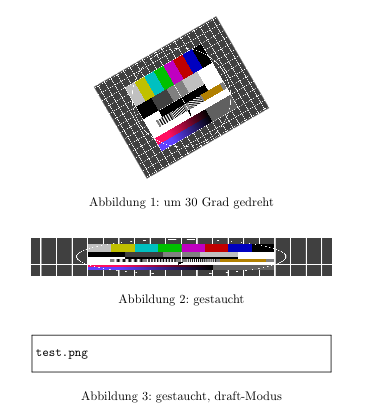
\includegraphics[height=1in,width=1in,angle=-90]{sections/08_Geometrie/pythagoras.standalone.pdf}
%\caption{This is a figure.}
%\end{center}
%\end{figure}

%\begin{figure}
%    \centering
%    \subfloat{
%	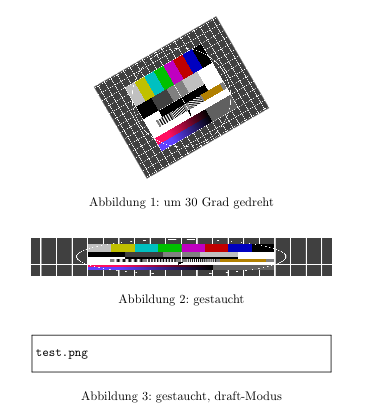
\includegraphics[height=2in,width=2in,angle=-90]{sections/08_Geometrie/pythagoras.standalone.pdf} 
%   }\hfill
%   \subfloat{
%      \begin{minipage}[t]{120mm}
%   	$A = \frac{d^2 \cdot \pi}{4}$ \\
%	$U = d \cdot \pi  $
%      \end{minipage}
%    }
%  \caption{Abbildungsname}
%  \label{fig:decision-tree}
%\end{figure}

\subsubsection{Kathetensatz}
%TODO picture
\begin{align*}
    a^2=c \cdot p \\
    b^2=c \cdot q \\
\end{align*}

\subsubsection{Trapez}
%TODO picture
\begin{align*}
    A &= \frac{a+b}{2} \cdot h = m \cdot h \\
    m &= \frac{a+b}{2}
\end{align*}

\subsubsection{Kreis}
%TODO picture
\begin{align*}
    A &= \frac{d^2 \cdot \pi}{4} \\
    U &= d \cdot \pi \\
\end{align*}

\subsubsection{Kreisausschnitt}
%TODO picture
\begin{align*}
    A &= \frac{d^2 \cdot \pi}{4} \cdot \frac{\alpha^\circ}{360^\circ} = \frac{b \cdot r}{2} \\
    b &= \frac{d \cdot \pi \cdot \alpha^\circ }{ 360^\circ} \\
\end{align*}

\subsubsection{Ellipse}
%TODO picture
\begin{align*}
    A &= \frac{D \cdot d \cdot \pi}{4} = a \cdot b \cdot \pi \\
    U &\approx \frac{D+d}{2} \cdot \pi \\
\end{align*}


\subsection{Stereometrie}
\paragraph{Gerade Körper}
\begin{align*}
    V = A \cdot h
\end{align*}

\paragraph{Spitze Körper}
\begin{align*}
    V = \frac{1}{3} \cdot A \cdot h
\end{align*}

\paragraph{Stumpfe Körper}
\begin{align*}
    V = \frac{1}{3} \cdot h ( A_1 + \sqrt{A_1 \cdot A_2} + A_2)
\end{align*}

\paragraph{Kugel}
\begin{align*}
    V &= \frac{4}{3} \cdot \pi \cdot r^3 \\
    O &= 4 \cdot \pi \cdot r^2 \\
\end{align*}

\subsection{Trigonometrie}
\subsubsection{Winkelfunktionen im rechtwinklichen Dreieck}
%TODO picture
\begin{align*}
    \sin \alpha &= \frac{\textrm{Gegenkathete}}{\textrm{Hypotenuse}}  &= \frac{a}{c} \\
    \cos \alpha &= \frac{\textrm{Ankathete}}{\textrm{Hypotenuse}}     &= \frac{b}{c} \\
    \tan \alpha &= \frac{\textrm{Gegenkathete}}{\textrm{Ankathete}}   &= \frac{a}{b} \\
    \cot \alpha &= \frac{\textrm{Ankathete}}{\textrm{Gegenkathete}}   & = \frac{b}{a} \\
\end{align*}

\paragraph{Trigonomische Beziehungen der Komplementwinkel}
\begin{align*}
    \sin \alpha &= \cos \beta  = \cos (90^\circ - \alpha) \\
    \cos \alpha &= \sin \beta  = \sin (90^\circ - \alpha) \\
    \tan \alpha &= \cot \beta  = \cot (90^\circ - \alpha) \\
    \cot \alpha &= \tan \beta  = \tan (90^\circ - \alpha) \\
\end{align*}


\subsubsection{Winkelfunktionen im spitz- und stumpfwinklichen Dreieck}


\paragraph{Sinussatz}
%TODO picture
\begin{align*}
    a : b : c = \sin \alpha : \sin \beta :\sin \gamma \\
    \frac{a}{\sin \alpha} = \frac{b}{\sin \beta} = \frac{c}{\sin \gamma}
\end{align*}

\paragraph{Kosinussatz}
%TODO picture
\begin{align*}
    a^2 = b^2 + c^2 -2bc \cos \alpha \\
    b^2 = c^2 + a^2 -2ca \cos \beta \\
    c^2 = a^2 + b^2 -2ab \cos \gamma \\
\end{align*}

\paragraph{Fläche eines Dreiecks}
\begin{align*}
    A = \frac{1}{2} ab \sin \gamma = \frac{1}{2} bc \sin \alpha = \frac{1}{2} ac \sin \beta
\end{align*}


\subsection{Geniometrie}
\subsubsection{Bogenmaß}
%TODO picture
\begin{align*}
    1  \textrm{ rad} = \frac{180^\circ}{\pi}        \\
    1 ^\circ = \frac{\pi}{180^\circ} \textrm{ rad}  \\
    x = \frac{b}{r} = \frac{\pi}{180^\circ} \cdot \alpha^\circ \\
\end{align*}

\subsubsection{Grundbeziehungen}
\begin{align*}
    \sin^2 \alpha + \cos^2 \alpha = 1 \textrm{ (Trigonomischer Pythagoras)} \\
    \tan \alpha = \frac{\sin \alpha}{\cos \alpha};
    \cot \alpha = \frac{\cos \alpha}{\sin \alpha};
    \tan \alpha \cdot \cot \alpha = 1
\end{align*}

\subsubsection{Winkelbeziehungen in den Quadranten}



\section{Vectorrechung}

\newcommand{\myvec}[3]{
\left(
    \begin{array}{c}
    #1 \\ #2 \\ #3
    \end{array}
\right)
}


\subsection{Darstellung}
$$
\vec{a}= \vec{a}_x +\vec{a}_y +\vec{a}_z = a_xi +a_yj + a_zk= \myvec{a_x}{a_y}{a_z}
$$

\subsection{Betrag}
$$
|\vec{a}|= a = \sqrt{a_x^2 +a_y^2 + a_z^2}
$$

\subsection{Einheitsvector}
$$
  \vec{a}_0 = \frac{\vec{a}}{|\vec{a}|}  \longrightarrow \vec{a}_0 \cdot \vec{a} = a \cdot \vec{a}
$$

\subsection{Addition}
\begin{align*}
  \vec{a} \pm \vec{b} &= (a_xi +a_yj + a_zk) \pm (b_xi +b_yj + b_zk)\\
  &= (a_x+b_x)i +(a_y+b_y)j + (a_z+b_z)k \\
  &=  \myvec{a_x \pm b_x}{a_y \pm b_y}{a_z \pm b_z}
\end{align*}

\subsection{Nullvector}
\begin{align*}
  \vec{a}-\vec{a}&= \vec{0} \\
  |\vec{0}|&=0
\end{align*}

\subsection{Multiplikation mit Skalar}
\begin{align*}
 n \cdot \vec{a} =   \myvec{n \cdot a_x}{n \cdot a_y}{n \cdot a_z}
\end{align*}

\subsection{Multiplikation von Vectoren (Skalarprodukt)}
\begin{align*}
 \vec{a} \cdot \vec{b} =  |\vec{a}| \cdot |\vec{b}| \cos{(\vec{a},\vec{b})}
\end{align*}


\subsection{Gesetze}
\begin{align*}
 \vec{a} \cdot \vec{b} = \vec{b} \cdot \vec{a} (assoziativ) \\
 n \cdot (\vec{a} \cdot \vec{b}) =  (n \cdot \vec{a}) \cdot \vec{b} = \vec{a} \cdot(n \cdot \vec{b})  (kommutativ) \\
 \vec{a} \cdot (\vec{b} \pm \vec{b}) = \vec{a} \cdot \vec{b} \pm  \vec{a} \cdot \vec{c} (distributiv) \\
\end{align*}

\subsection{Sonderfall}
\begin{align*}
 \vec{a} \cdot \vec{a} &= |\vec{a}| \cdot |\vec{a}| \cdot \cos 0^\circ \\
 &=  \vec{a}^2 = a^2
\end{align*}

\subsection{Kreuzprodukt}
\begin{align*}
 \vec{a} \times \vec{b} &= \left|
                               \begin{array}{ccc}
                                  i & j & k \\
                                  a_x & a_y & a_z \\
                                  b_x & b_y & b_z \\
                               \end{array}
                               \right|\\
                         =   \left|
                              \begin{array}{ccc}
                                 a_y & a_z  \\
                                 b_y & b_z \\
                              \end{array}
                              \right|i + \\
                              \left|
                              \begin{array}{ccc}
                                 a_z & a_x  \\
                                 b_z & b_x \\
                              \end{array}
                              \right|j + \\
                             \left|
                             \begin{array}{ccc}
                                a_x & a_y  \\
                                b_x & b_y \\
                             \end{array}
                             \right|k
\end{align*}

\subsection{Spatprodukt}
\begin{align*}
 \vec{a} \cdot \vec{b} \cdot \vec{c} &=    \left|
                                           \begin{array}{ccc}
                                              a_x & a_y & a_z \\
                                              b_x & b_y & b_z \\
                                              c_x & c_y & c_z \\
                                           \end{array}
                                           \right|\\
\end{align*}






\section{Matrixrechnung}
 $$
\Sigma=\left[
\begin{array}{ccc}
   \sigma_{11} & \cdots & \sigma_{1n} \\
   \vdots & \ddots & \vdots \\
   \sigma_{n1} & \cdots & \sigma_{nn}
\end{array}
\right]
$$

 $$
\Sigma=\left(
\begin{array}{ccc}
   \sigma_{11} & \cdots & \sigma_{1n} \\
   \vdots & \ddots & \vdots \\
   \sigma_{n1} & \cdots & \sigma_{nn}
\end{array}
\right)
$$


\newcommand*{\rowvec}[1]{\left( #1\right)}
\newcommand*{\rowvecVert}[1]{\left(\begin{array}{c}#1\end{array}\right)}

$$
\rowvec{1,2,3}
$$

$$
\left(
\begin{array}{c}
1 \\ 2 \\ 3
\end{array}
\right)
$$
$$
\vec{B} = \rowvecVert{1 \\ 2 \\ 3}
$$
\section{Stochastik}
\subsection{Wahrscheinlichkeit}
TBD
\subsection{Statistik}
TBD


\section{Konstanten}
\begin{align*} 
\pi =  4 \cdot \sum_{n=0}^\infty  \frac{(-1)^n}{2n+1} = \frac{1}{1} -  \frac{1}{3} +  \frac{1}{5} -  \frac{1}{7} + \frac{1}{9} \mp ... = \textbf{3,14159}...
\end{align*}
\begin{align*} 
e = 1 + \frac{1}{1}+\frac{1}{1 \cdot 2}+\frac{1}{1 \cdot 2  \cdot 3}+\frac{1}{1 \cdot 2  \cdot 3  \cdot 4}+... = \sum_{k=0}^\infty \frac{1}{k!} = \textbf{2,71828183}...
\end{align*}


\section{Zeichenerklärung}

\begin{tabular}[h]{l|l}
Zeichen &Bedeutung  \\
\hline
$\widehat{=}$ & entspricht  \\
$\longrightarrow$ & daraus folgt \\
$\sum$ & Summenzeichen \\
$\prod$ & Produktzeichen \\
$\in$ & Element von \\
$\notin$ & nicht Element von \\
$|$ & mit der Bedingung \\
$\land$ & und \\
$\lor$ & oder \\
$\lnot$ & nicht \\
$\infty$ & Unendlich \\

\end{tabular}





\end{document}
% ======================= END

$ \to $ % daraus folgt

$$\frac{a \pm b}{c} =  \frac{a}{c} \pm \frac{b}{c} $$

$\frac{a \pm b}{c} =  \frac{a}{c} \pm \frac{b}{c} $



